\newpage
\subsection{Survey}

\subsubsection{Goal of the Survey}
The goal of this qualitative survey was to gather in-depth data about designer-developer
collaboration patterns and identify key friction points in their workflows.

\subsubsection{Survey Design}
Although the survey was designed to be answered by both designers and developers, the questions were
tailored to their fields. After an initial question about their role, the survey branched into two
paths. One for designers and one for developers. While the structure and order of the questions
remained similar, the wording and focus of some was slightly adjusted. The thought behind that was
to make it easy for both parties to answer, while being able to compare and align the responses
later on.

Examples of questions include: % NOTE DONE: show them in a better way than a table... Nah Table is ok
\begin{center}
    \begin{tabular}{|m{7.5cm}|m{7.5cm}|}
        \hline
        \textbf{Designer Question}                                                                         & \textbf{Developer Question}                                                                                \\
        \hline
        How would you rate your understanding of web development?                                          & How comfortable are you working with design tools like Figma?                                              \\
        \hline
        What do you think were the main reasons for these discrepancies between design and implementation? & What issues do you commonly face with design handoffs and implementing designs?                            \\
        \hline
        When making a new version [\dots], how do you communicate these changes to the developers?         & When a component needs to be changed, [\dots] how do you expect the designer to communicate these changes? \\
        \hline
    \end{tabular}
\end{center}

Formulating the questions in this way allowed for seeing if there are any discrepancies in the
workflow and how expectations align. The majority of questions were multiple choice, with some
open-ended ones to allow for some more reflective answers. Also, the survey included custom graphics
and a hint of humor to make it more engaging.
\begin{figure}[H]
    \centering
    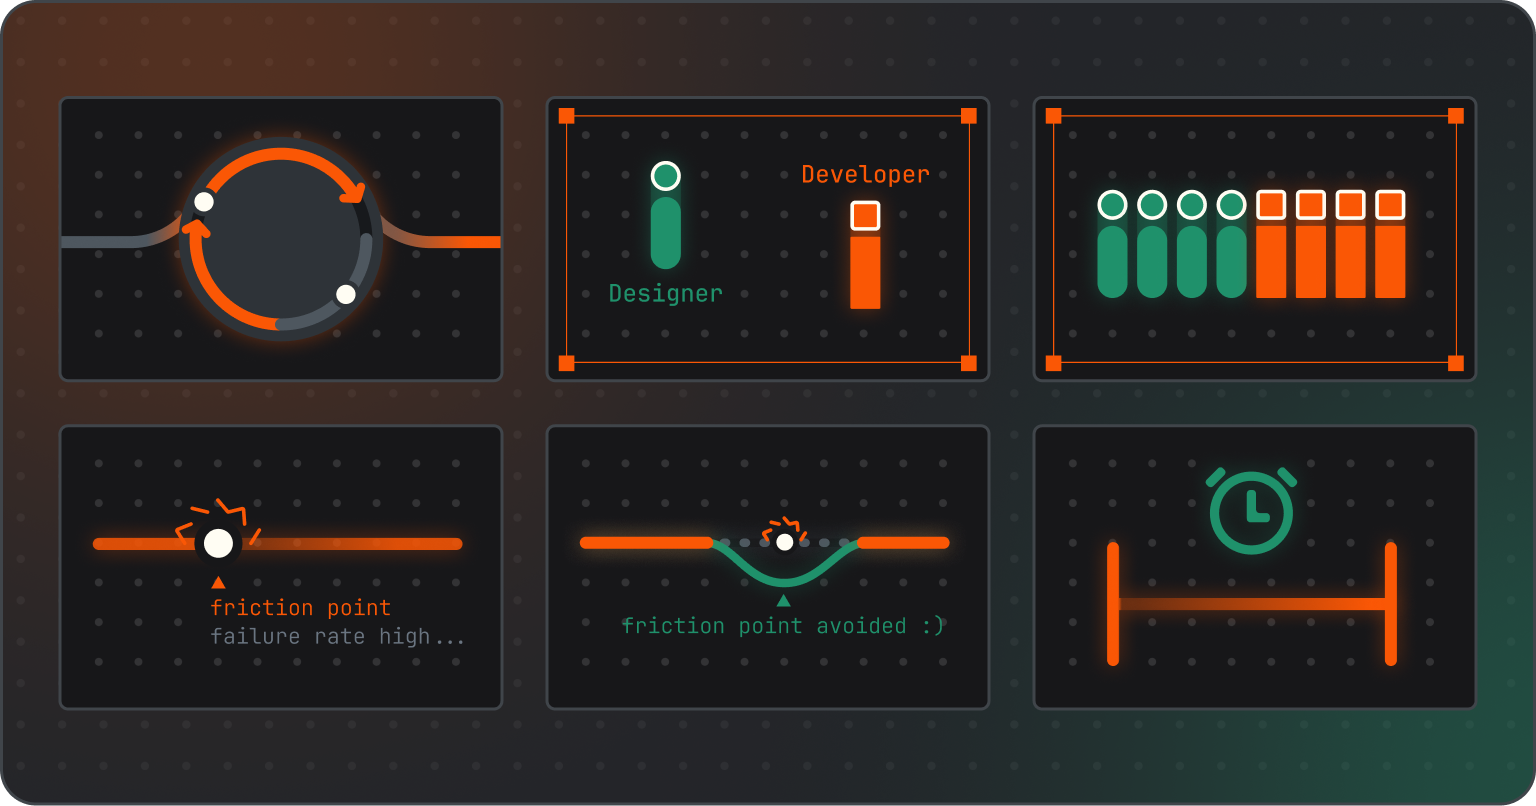
\includegraphics[width=300pt]{Chapter 4/Survey Pics.png}
    \caption{Custom survey graphics (Source: own illustration)}
\end{figure}
% NOTE DONE: show the graphics specially made for the survey

As the survey was designed to reach both beginners and experienced professionals, the survey was
distributed to a wide range of channels:
\begin{itemize}
    \item Two small web development companies with a focus on design
    \item A list of Design and Software Development students at FH Joanneum
    \item LinkedIn connections
    \item Personal designer and developer contacts
\end{itemize}

\subsubsection{Presentation of Survey Results}
\begin{figure}[H]
    \centering
    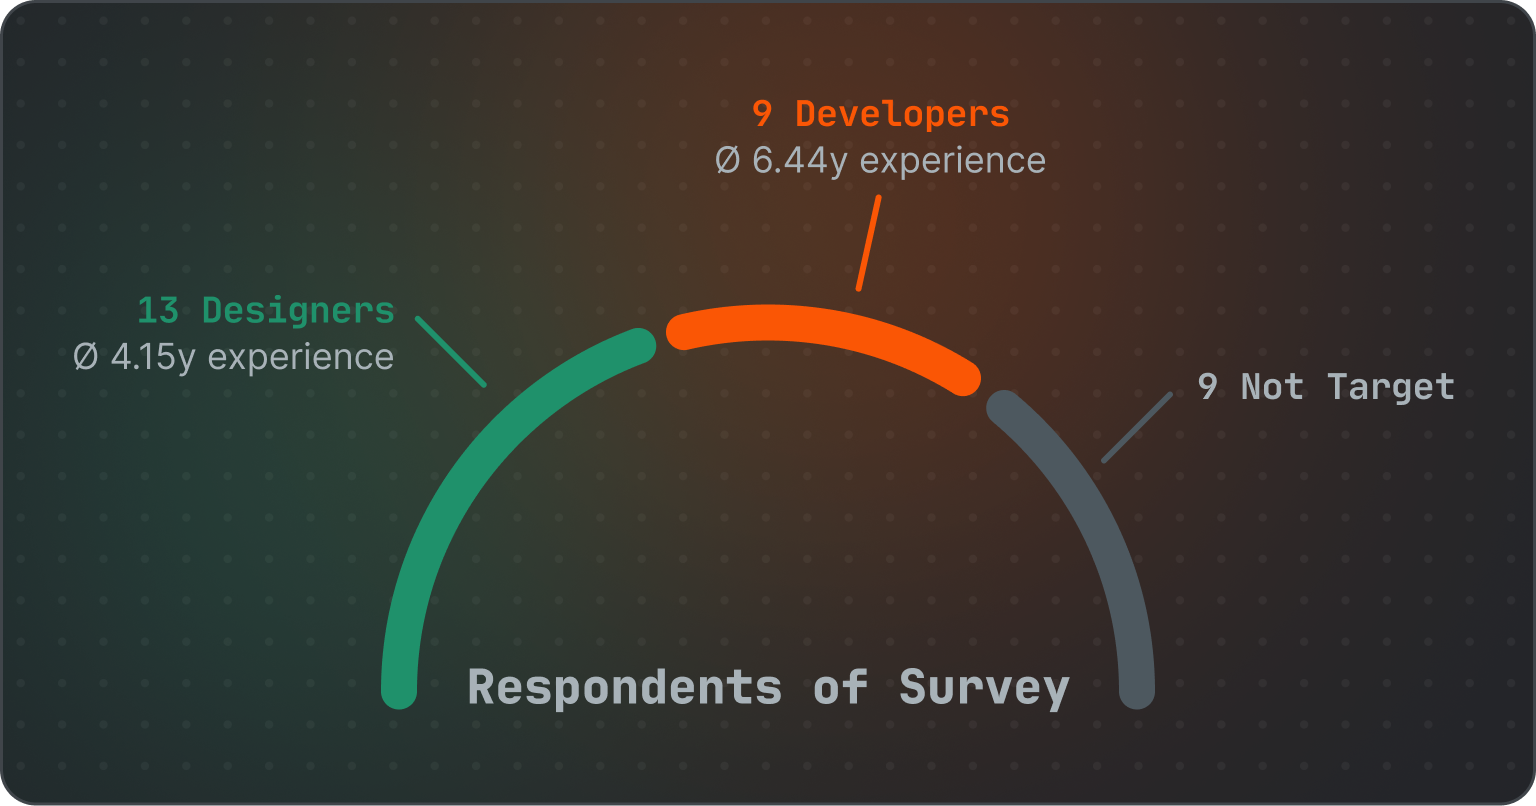
\includegraphics[width=300pt]{Chapter 4/Respondents.png}
    \caption{Respondents of Survey (Source: own illustration)}
\end{figure}
Over a duration of 30 days, 31 people responded to the survey. 13 of which considered themselves
primarily as designers, 9 as developers and 9 were not in the target group. While the sample size is
small, the results are qualitative and provide valuable insights and perspectives.

The majority of designers have not yet had as many years of professional experience as the
developers.
% NOTE DONE: Show some numbers here, bar graphs with two bars (one for designer one for developer could
% be suitable here)

The survey supported online claims of Figma being the most popular design tool. 85\% of designers
said they use Figma for designing interfaces. Tools like Photoshop are still used by 25\% as
secondary tools.

\textbf{Knowledge of the other discipline:}\\
\begin{figure}[H]
    \centering
    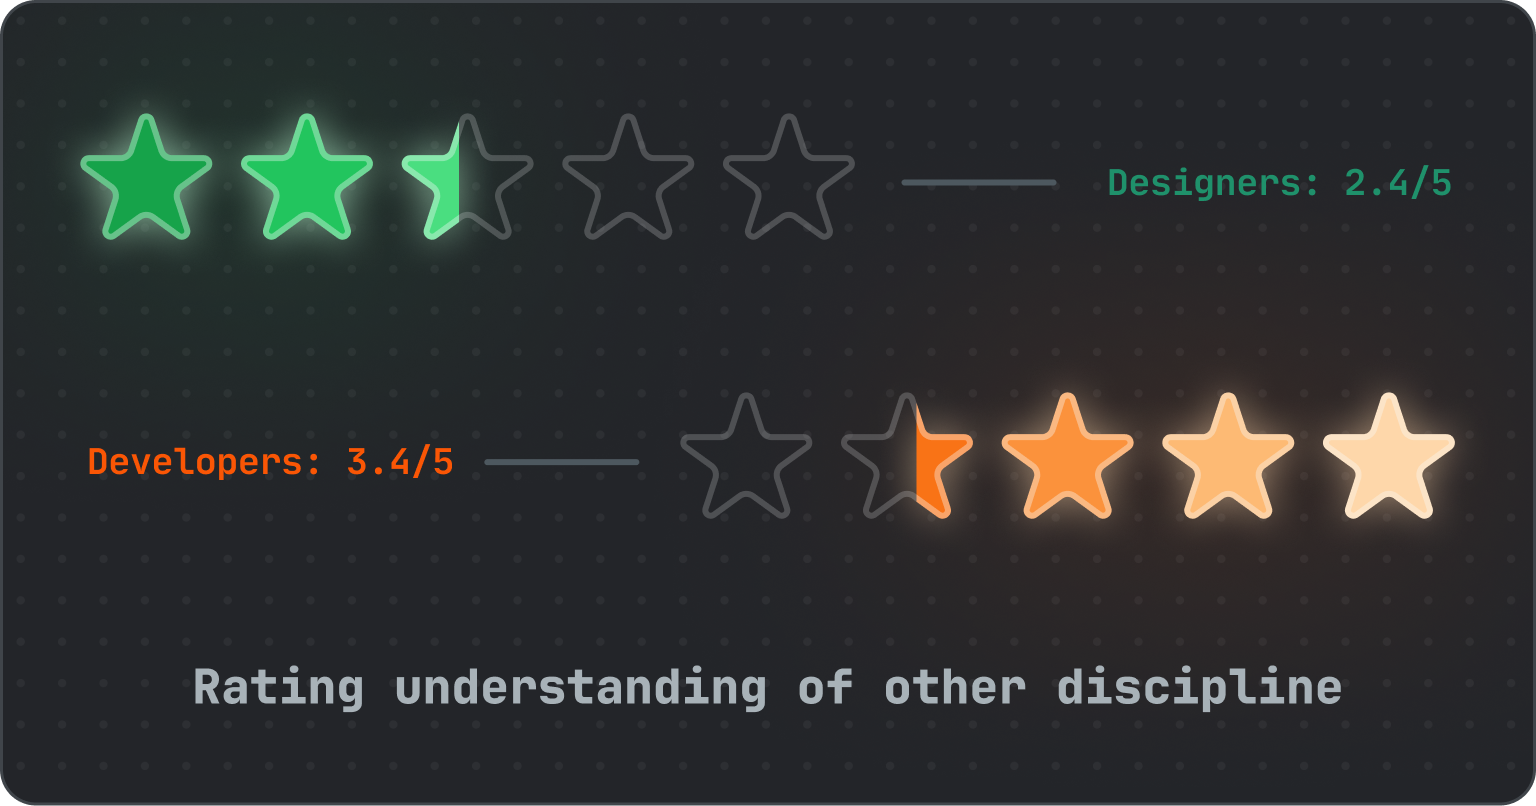
\includegraphics[width=300pt]{Chapter 4/Rating.png}
    \caption{Rating understanding of other discipline (Source: own illustration)}
\end{figure}
When asked about their understanding of the other discipline, the majority of designers rated their
web development knowledge at 3/5 stars, knowing the basics of HTML, CSS and JavaScript. 2 of
them even rated it as "5/5 stars - Honestly could do the developers job :)". Also Developers seem to
know their way around design tools like Figma with 75\% rating their comfort level as 3/5 or higher.
Responses suggest that while there is a general understanding of the other disciplines tools, there
is room for improvement.

\textbf{Discrepancies between Design and Implementation:}\\
81\% of designers said they have experienced discrepancies between design and implementation. The
most common reasons being time constraints, misinterpretation by developers and "Special cases like
complex animations, Popups, Microinteractions". When asked about the main issues with design
handoffs, developers claimed that "Too few designed states (missing hover, focus, \dots)" and
the unclarity of responsive layouts were the most common. Noteworthy is also that devs think complex
components as well as animations, popups or modals are often not well enough specified or
documented. Furthermore, designs not having a component-based approach seem to be a problem, despite
over 80\% of designers claiming they work with such an approach.
These results suggest that there is a common ground for persisting issues. While designers seem to
be aware of component-based design, there may be a misalignment in how it is understood between
disciplines.
% NOTE: In discussion mention that maybe the designers should learn component based design a little
% better or that they should learn how to structure them better

\textbf{Communication:}\\
Despite none of the engineers thinking that "lack of communication with designers" is a re-occurring
issue, some designers state that "more time together with developer[s] and clear communication"
would be beneficial for the workflow.

Regarding practices that have improved the designer-developer collaboration, the most frequent
mentioned factors were proper documentation, design systems, well-structured components and early
involvement of developers. One developer noted that best results were achieved when the disciplines
tried to work out solutions together:
"Implementing a collaborative approach early on in projects: Continuous check-ins with designers and
developers to find the best solution within the given target, budget, and timeline."

\begin{figure}[H]
    \centering
    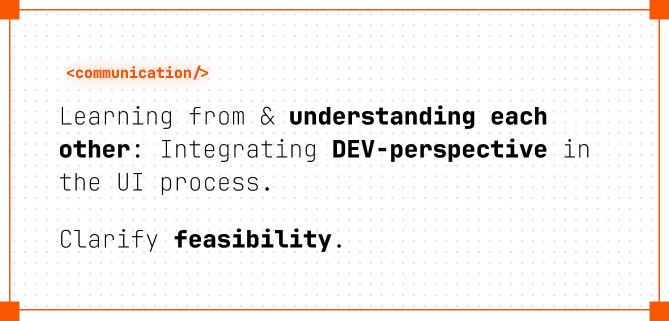
\includegraphics[width=300pt]{Chapter 4/Quote Communication.png}
    \caption{Survey quote on communication (Source: own illustration)}
\end{figure}
% NOTE DONE: Add Quote here

\textbf{Bad and Good Practices:}\\
Respondents identified several specific bad practices that they would like to see less of in the
future. Here, the most commonly named was that there are too many different components and variants
where it is not needed, with one dev recognizing that maybe designers and developers have a
different understanding of what a component is: "Having similar components in thousands of variants
is the default mode in design tools, while in development having few components with a few variants
is the default". Also "inconsistency throughout repeating patterns" were mentioned as a common
practice as well as not using the already designed or developed components. These results shows
again that a diverging understanding of components may be present and that design systems are not
yet used to their full potential.

On the other hand, helpful practices mentioned by the engineers include using clearly defined design
tokens, fonts and colors consistently as well as defining edge-case behaviours and annotating
components. \\

Building on these findings, the next section discusses the underlying causes and possible solutions
to these problems.

\subsubsection{Discussion \& Conclusion}
% Points to discuss
% - Misunderstanding of components: Designers as well as developers often find themselves asking "Should
%   this be a new component or a variant of an existing one? Or is this not a component after all?".
%   Even in the coding world there are different best practices how to structure components. So, it
%   probably is best to ask the team and agree on some basic guidelines. The basic rule of thumb is
%   if a part of a design is used more than once, it should be a component. Also maybe design tools
%   somehow encourage the craetion of too many components as it is very easy to create a component
%   in Figma. Variants are also very powerful, but should only be used to group together different
%   styles of the same component. This would also lead to a closer design and code parity, since in
%   code this is handled very similarly. (<Button variant="primary" size="large">)

% - Unclear layouts: It seems as though responsive layouts are often not well enough defined. Maybe
%   this is due to the fact that designers are working in a pretty fixed setting. Devs can drag the 
%   browser window easily to see how the design behaves. Also, defined grids are pretty rigid and
%   devs often have a hard time to make them work responsively. A proper definition of how grids
%   behave in different breakpoints could definitely help there => Devs use defined breakpoints,
%   designers should use the same ones to define how the design should behave at those specific
%   breakpoints. Also

% - Time Constraints: It seems as though the time constraints cause a lot of issues. Often
%   documentation and proper definition of edge cases as well as hover, empty states are left out.
%   Maybe prioritizing these aspects more could help. Also maybe doing handoffs more often and in
%   smaller batches like Agile workflows suggest could be helpful, as the developers wouldn't need
%   to wait for the whole design to be finished without proper documentation, but could start
%   working sooner with the parts that are already properly defined. Team working agreements can
%   help with that (Lean UX page 87)

% - Conclusion:
% NOTE: Design and Code Parity: https://designsystemdiaries.com/p/figma-to-code-design-system-parity

A common theme throughout the survey was the misalignment in understanding components. It seems as
if designers and developers are using components a little differently, despite using the same
nomenclature. One of the most frequently asked questions in both disciplines is whether an element
should be a new component, a variant of an existing one, or not a component at all. Although there
are different best practices for structuring components in code, the basic rule of thumb is that if
a part is used more than once, it should be a component. The same could simply be done in design
tools. Variants should be used to group components that use the same properties like layout, state,
size, count or others as Figma suggests. \vglcite{figmaCreatingOrganizingVariants2025}

Generally, establishing some basic guidelines for the team helps to improve design-code parity as it
is possible to have a similar structure in both code and design.
\begin{figure}[H]
    \centering
    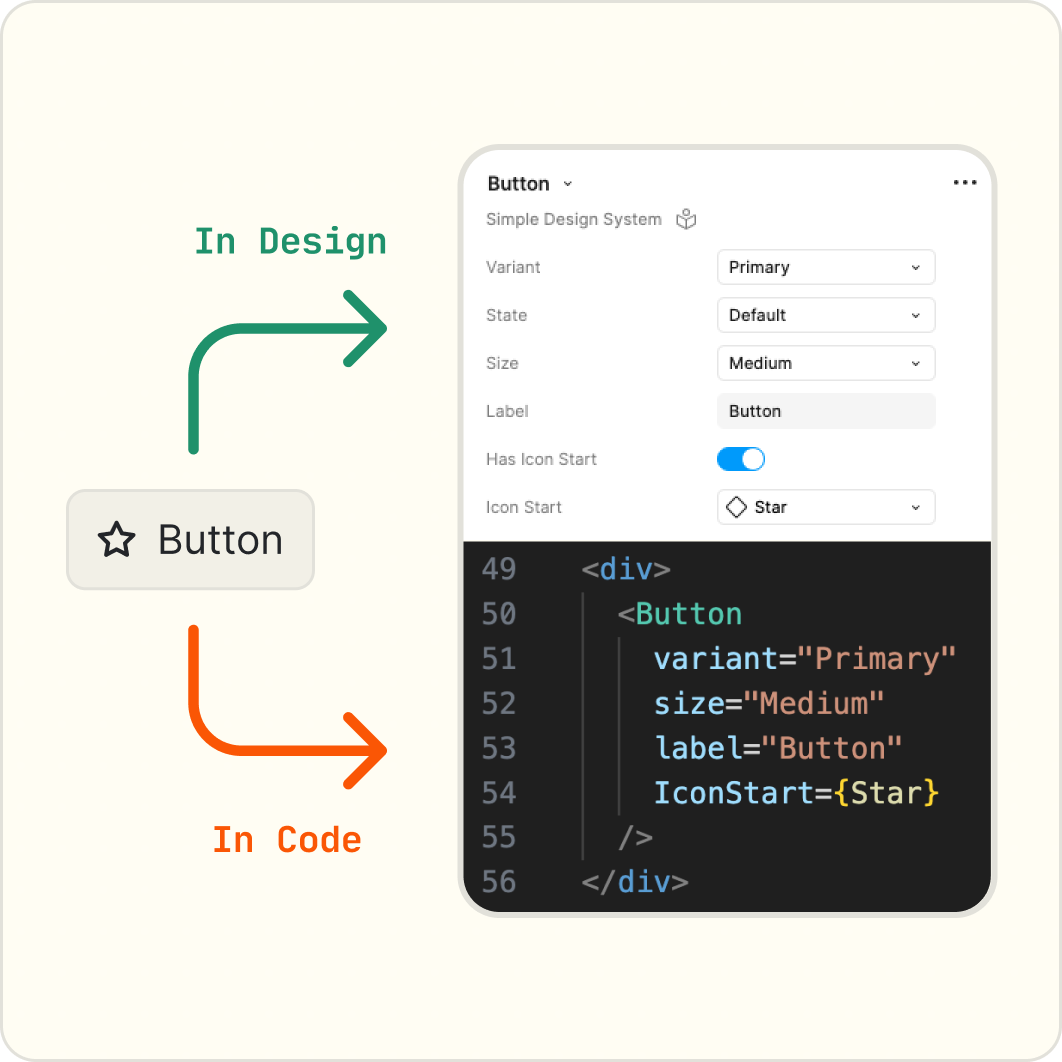
\includegraphics[width=300pt]{Chapter 4/DesignCode Parity.png}
    \caption{Design-Code parity illustrated (Source: own illustration)}
\end{figure}
% NOTE DONE: Graphics of design and code parity with like idk <Button variant="primary" size="large"> 

Another frequently mentioned issue was the unclear definition of responsive layouts. While design
tools often work in a rather fixed setting, developers can easily switch their viewport to see how
the design behaves. While grids can already be helpful for both, sometimes sizings are hard to
interpret for developers. When setting up desktop, tablet and mobile grids, it is important to agree
on universal breakpoints used by both groups. Furthermore, defining a number of simple page layouts
with specified maximum and  minimum sizes for certain elements like navigation and content can be
extremely beneficial.
% NOTE: Maybe I can have the spacing shizzle I defined for EA: Nö leider
This way, developers can implement grids more easily without guesswork and even designers benefit as
they can take these defined layout grids as a starting point for page designs. Also, defining tablet
and mobile versions of components directly next to each other can help the developers to quickly
implement and quality check the design.

These suggested practices also improves the consistency of repeating patterns, which was another
problem mentioned in the survey. Design tokens like colors, fonts and spacings also fit into the
same category, although they seem to be managed quite well by designers already.

Lastly, time constraints seem to be the root cause to many smaller details. Tasks that are done late
in the process like documentation, definition of edge cases, empty states or focus states come short
when there is no time left. While teams may not be in control of the deadlines, they can change how
they work together. As described in chapter \ref{Agile Project Management & Lean UX}, working in an
Agile manner with smaller handoffs and much more frequent check-ins can boost the workflow. With
smaller handoffs, it may be possible to prioritise documentation, edge cases and other details more
consistently and earlier in the process.

Lean UX further suggests that teams should create a so-called \textit{Team Working Agreement} to
define how they want to work together. This includes development practices, requirements for design,
working hours and more and is refined with each retrospective meeting.
\vglcite[87, 89]{gothelfLeanUXProduktentwicklung2016}

This concludes my analysis of the survey results. Although, the sample size is small, the insights
are valuable and serve as a great foundation for the practical part of this thesis. To make sure the
practical work is based on as much research as possible, two additional interviews have been
conducted and summarized in the next chapter.
